
\chapter{評価}
\label{evaluation}
第\ref{implementation}章にて述べたシミュレータを用いて,本提案手法の妥当性を検証するための評価実験を行う.
本章では評価実験の概要と,それにより得られた結果及び考察について述べる.
\section{仮定}
本節に本評価実験の仮定条件となる事項を記述する.

\subsection{運用環境のモデルケース}
\label{model-case}
\ref{purpose-proposal}節で述べたように,本研究の提案手法では以下のような環境の駐車場を想定している.
\begin{itemize}
	\item 駐車場全体が広く,区画の空き状況を利用者が一度に確認することが困難である.
	\item 駐車区画の人気度に偏りがある.
	\item 運営者による満空情報の開示が難しい.
\end{itemize}

本論文ではそれらに当てはまるモデルケースとして,慶應義塾大学湘南藤沢キャンパス(以後SFC)の各駐車区画を本シミュレータ上に再現した.各駐車区画の座標,座標間の距離はGoogleMaps\cite{googlemap}より参照した.図\ref{google-sfc}にGoogleMaps上にプロットしたSFCのネットワークモデルを示す.評価実験を明確にするために一部を簡略化している.

\begin{figure}
	\centering
	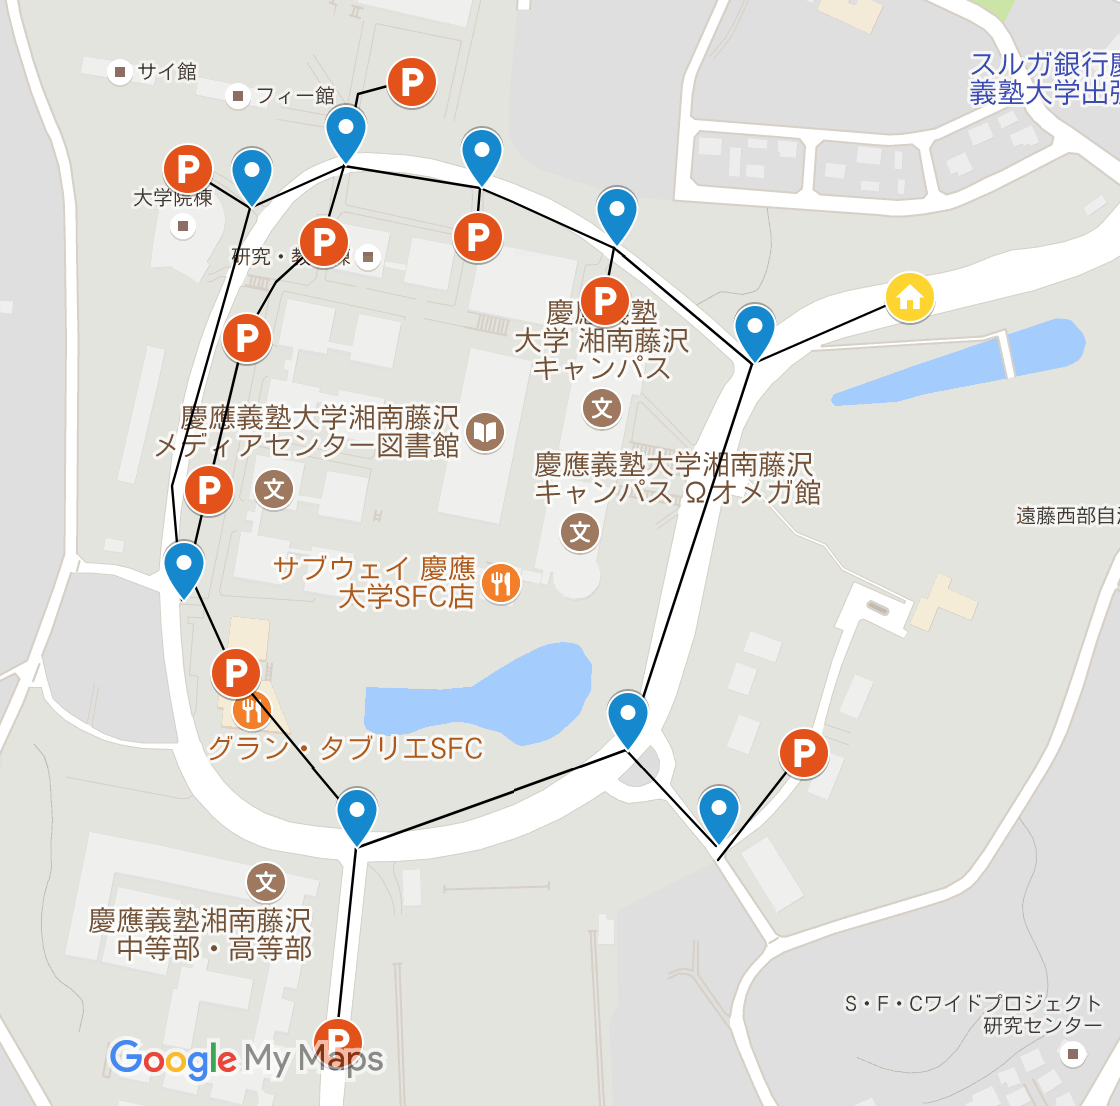
\includegraphics[width=10cm]{fig/google-map.png}
	\caption{googleMaps上にプロットしたSFC内駐車区画のネットワークモデル}
	\label{google-sfc}
\end{figure}


図\ref{sfc-network-model}が本ミュレーター上に再現したSFCのネットワークモデルである.駐車区画を$P$,その他の道路との接続点を$C$としている.車両が駐車場内に進入する箇所を0として,それぞれ19まで識別コードを割り当てる.

\begin{figure}
	\centering
	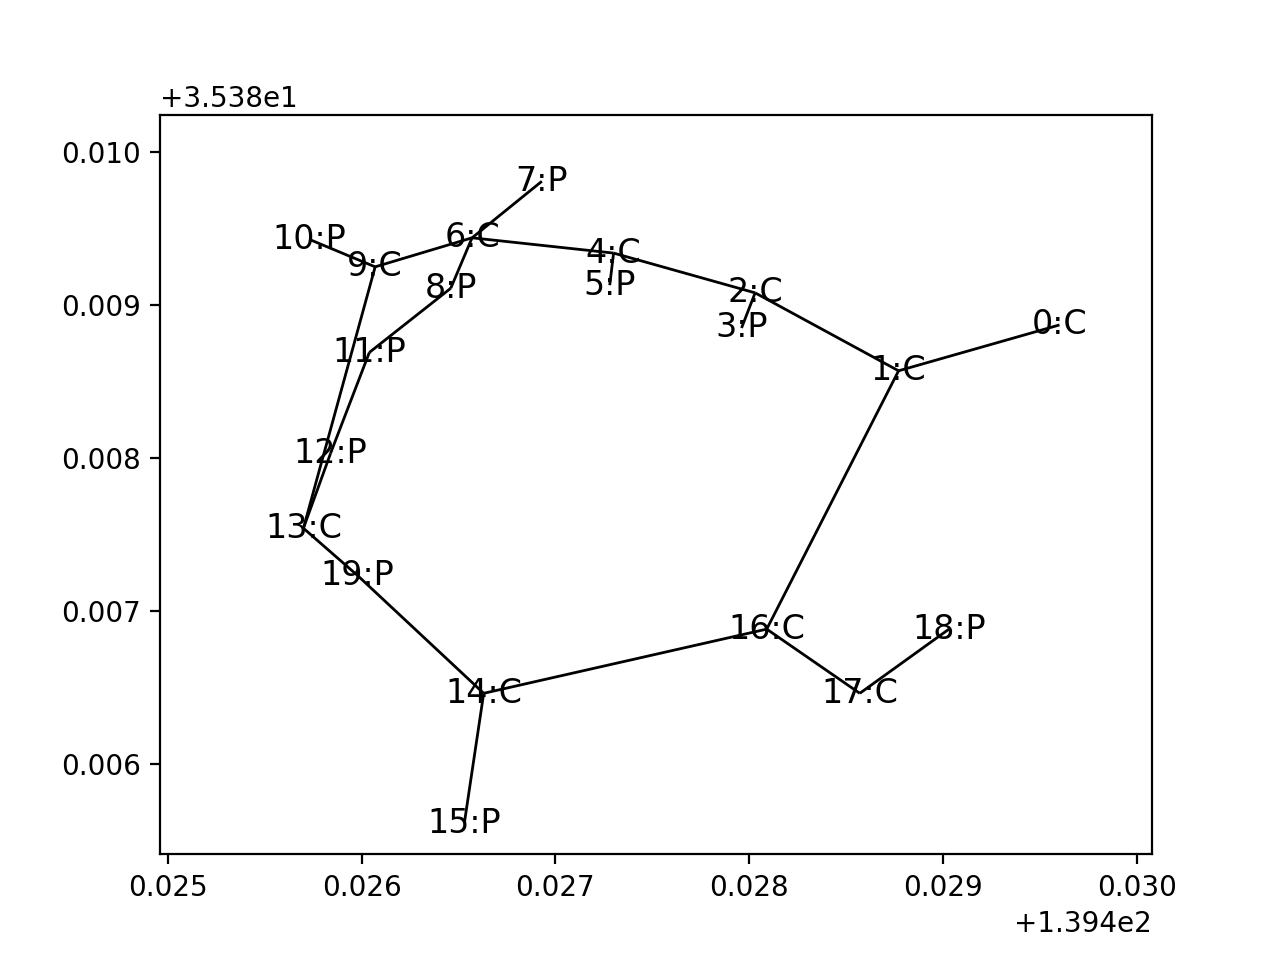
\includegraphics[width=12cm]{fig/place-sfc.png}
	\caption{ネットワークモデル化したSFC}
	\label{sfc-network-model}
\end{figure}

\subsubsection{各ネットワークノードの特徴}
本評価実験において,各ネットワークノードの駐車枠数や特徴,各駐車場の人気度などは以下の表\ref{sfc-nodes}の通り指定する.
なお,各駐車区画の有する駐車枠数は2018年1月に実施した予備調査で計数したもの,人気度は任意に設定したものである.

\begin{table}[htbp]
	\centering
	\resizebox{\textwidth}{!}{%
		\begin{tabular}{lccclll}
			\hline
			\multicolumn{7}{c}{本評価実験における各ネットワークノードの特徴} \\ \hline
			\multicolumn{1}{c|}{Place ID} & 駐車場 & \multicolumn{1}{l}{駐車枠数} & \multicolumn{1}{l}{人気度} & 座標{[}緯度,経度{]} & 隣接するノードと距離{[}m{]} & 備考                             \\ \hline
			\multicolumn{1}{l|}{0}        & ×        & -                                & -                             & 35.38887,139.4296         & 1:82                                  & スタート地点                 \\
			\multicolumn{1}{l|}{1}        & ×        & -                                & -                             & 35.38857,139.42877        & 0:82,1:82                           &                                    \\
			\multicolumn{1}{l|}{2}        & ×        & -                                & -                             & 35.38908,139.42803        & 1:82,3:26,4:72                    &                                    \\
			\multicolumn{1}{l|}{3}        & ○       & 14                               & 10                            & 35.38885,139.42796        & 2:26                                  & アルファ館横                 \\
			\multicolumn{1}{l|}{4}        & ×        & -                                & -                             & 35.38934,139.4273         & 2:72,5:23,6:67                    &                                    \\
			\multicolumn{1}{l|}{5}        & ○       & 16                               & 5                             & 35.38913,139.42728        & 4:23                                  & シータ館$\cdot$メディア館 \\
			\multicolumn{1}{l|}{6}        & ×        & -                                & -                             & 35.38944,139.42657        & 4:67,7:61,8:39,9:50             &                                    \\
			\multicolumn{1}{l|}{7}        & ○       & 80                               & 5                             & 35.38981,139.42693        & 6:61                                  & 体育館前                       \\
			\multicolumn{1}{l|}{8}        & ○       & 7                                & 20                            & 35.38911,139.42646        & 6:39,11:61                          & ラムダ館横                    \\
			\multicolumn{1}{l|}{9}        & ×        & -                                & -                             & 35.38925,139.42607        & 6:50,10:37,13:197                 &                                    \\
			\multicolumn{1}{l|}{10}       & ○       & 16                               & 15                            & 35.38943,139.42573        & 9:37                                  & タウ館横                       \\
			\multicolumn{1}{l|}{11}       & ○       & 14                               & 25                            & 35.38869.139.42604        & 8:61,12:76                          & イオタ館,オミクロン館  \\
			\multicolumn{1}{l|}{12}       & ○       & 14                               & 10                            & 35.38803,139.42584        & 11:76,13:56                         & カッパ館,イプシロン館  \\
			\multicolumn{1}{l|}{13}       & ×        & -                                & -                             & 35.38754,139.4257         & 9:137,12:56,19:43                 &                                    \\
			\multicolumn{1}{l|}{14}       & ×        & -                                & -                             & 35.38646,139.42663        & 15:95,16:140,19:104               &                                    \\
			\multicolumn{1}{l|}{15}       & ○       & 14                               & 30                            & 35.38561,139.4265         & 14:95                                 & 南門警備室前                 \\
			\multicolumn{1}{l|}{16}       & ×        & -                                & -                             & 35.38688,139.42809        & 1:198,14:140,17:94                &                                    \\
			\multicolumn{1}{l|}{17}       & ×        & -                                & -                             & 35.38646,139.42857        & 16:64,18:67                         &                                    \\
			\multicolumn{1}{l|}{18}       & ○       & 23                               & 15                            & 35.38688,139.42903        & 17:67                                 & テニスコート前              \\
			\multicolumn{1}{l|}{19}       & ○       & 24                               & 5                             & 35.38723,139.42598        & 13:43,14:104                        & 生協棟前                       \\ \hline
		\end{tabular}%
	}
	\caption{SFCの仮想地図内における各区画の属性}
	\label{sfc-nodes}
\end{table}

\subsection{条件設定}
\label{evaluation-test-conditions}
本評価実験の際に設定する条件について記述する.

\begin{itemize}
	\item 1シーケンスの時間 \\
	      本実装では1シーケンスを1秒($t = 1[秒]$)とする.これは利用車両の位置情報送信間隔を1秒と定義することに等しい.
	\item 各仮想車両の目的地の決定\\
	      本シミュレータでは車両が目的の区画で駐車が出来ない場合,他の区画を次の目的地として設定して場内を巡回する.その時,車両は通過した駐車区画に関してその区画の満空状況を確認出来るものとする.また,目的地ではない場合も車両ごとに定められた確率($Car$クラスの$confuse$プロパティ)に依って駐車を試みる.
	\item 仮想車両の駐車時間 \\
	      本評価実験では車両の駐車時間$p_t$は,1時間から3時間($3600[秒] < p_t < 10800[秒]$)までの任意の時間とする.
	\item 各駐車区画の人気度\\
	      各駐車区画の人気度は表\ref{sfc-nodes}で定めたものとする.
	\item 道路$\cdot$交差点の交通量のキャパシティ \\
	      本評価実験では各道路に収容できる交通量を制限しないものとする.仮想車両群は各駐車区画を無制限に通過することが出来る.一方で,区画が保有する駐車枠に空きが無い場合は,駐車を行わず通過するものとする.
	      	
	\item 位置情報ログの生成 \\
	      多様なパターンに対応するため,試行の度にシミュレータを実行し,仮想車両群の位置情報ログデータを生成する.
	\item 試行回数 \\
	      本評価実験では,変数を変える度にシミュレータの実行$\cdot$ネットワークモデルの推定を各説明変数につき100回ずつ行う.
	\item 座標の誤差 \\
	      車両から送信される位置情報に対して第\ref{implementation-send-position}項で述べた誤差付与処理を施す.生成される誤差の分布に関しては図\ref{error-kde}を参照されたい.
	      	
\end{itemize}


\section{評価実験}
\label{evaluation-test-about}
本提案手法の妥当性を検証するために2つの評価実験を行った.本節ではその概要と結果及び考察について述べる.
\subsection{評価実験1:駐車区画の位置推定}
\label{evaluation-test-1}
本項では,第\ref{how-to-park-area}節で述べた駐車区画の位置推定手法を,定量的に評価するための評価実験1について記述する.
\subsubsection{条件と変数}
評価実験1では第\ref{evaluation-test-conditions}節に挙げた条件の他に,以下のような条件を設定する.
\begin{itemize}
	\item 仮想車両のスタート方法\\
		すべての車両を同時にスタート地点から仮想地図内に進入させる.
	\item 最大シーケンス数(収集対象時間) \\
	      評価実験1では最大シーケンス数を設定しない.すべての車両が駐車を完了しSFCから退出するまでの位置情報ログを推定に用いる.
	\item 車両の数\\
	      \ref{evaluation-test-1-var}項に後述するように,評価実験1では仮想地図内に進入する車両の台数を説明変数とする.本実験での車両台数は,実環境下での利用車両の述べ台数とみなすことが出来る.
\end{itemize}
\subsubsection{評価項目}
\label{evaluation-test-1-eval-elements}
評価実験1では,以下の2項目に関して順に推定結果を検証し,推定の成功の可否を検証する.
\begin{enumerate}
	\item 駐車区画の数 \\
	      システムが推定した駐車区画の数と,真値の駐車区画の数が一致するかどうかを検証する.一致した場合次の項目に進む.
	\item 駐車区画の座標 \\
	      システムが推定した各駐車区画の座標群と,真値の座標群との距離が真値の駐車区画間の最短距離より小さい場合,推定が成功したと判断する.
\end{enumerate}

\subsubsection{説明変数と目的変数}
\label{evaluation-test-1-var}
評価実験1では説明変数$x$を仮想地図内に進入する台数とし.推定結果の成功率$y$を目的変数とする.$n$回試行した時の成功率$y$は以下の式のように表される.

なお,本システムの推定機構$f(x)$は推定が成功した場合1を,失敗した場合0を返す.

また,本実験では$x = 50,100,150,200,250,300,350,400,450,500,550,600$,$n=100$とする.

\begin{align}
	y = \frac{\sum_{i=1}^{n} f(x)}{n},x = 車両の台数 \\
	f(x) = 本システムの推定機構                 \\
	n = 総試行回数                                   
\end{align}



\subsubsection{結果}
$x=250$の一度の試行を例に,試行が成功した場合($f(x) = 1$)に,システムが推定した駐車区画の座標とクラスタリング処理を施した駐車時の座標群をプロットした結果を図\ref{evaluation-test-1-success}に示す.青い円は真値の駐車区画座標,線群は真値のネットワークモデルの道路を表すエッジである.

\begin{figure}
	\centering
	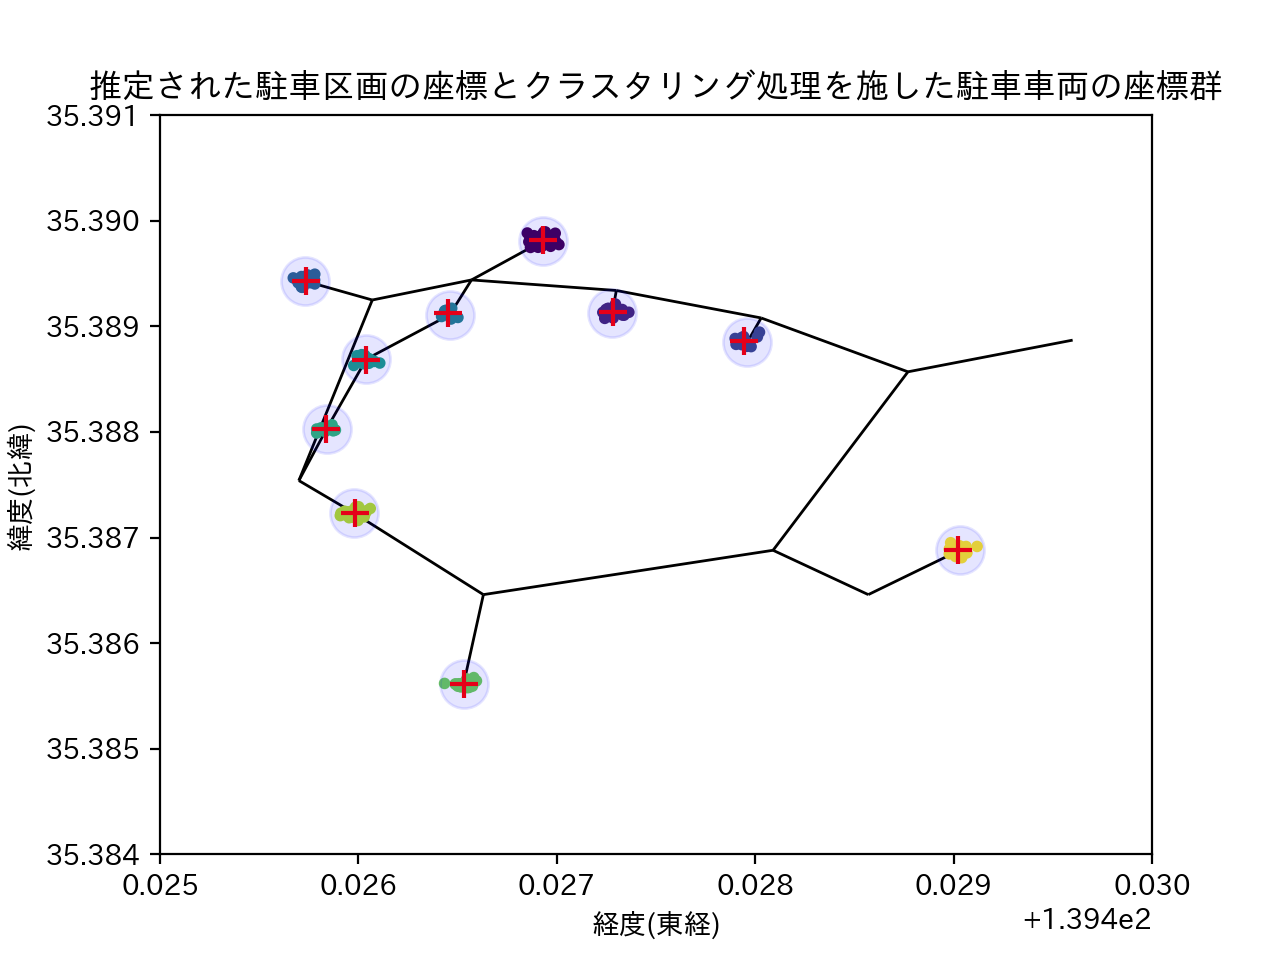
\includegraphics[width=14cm]{fig/eval-test-1-success.png}
	\caption{評価実験1が成功したケースにおける推定された駐車区画座標と真値の比較}
	\label{evaluation-test-1-success}
\end{figure}

評価実験1の結果を図\ref{evaluation_test_result_figure}に示す.$x>450$の場合に成功率が$90\%$を超えていることが読み取れる.
\begin{figure}
	\centering
	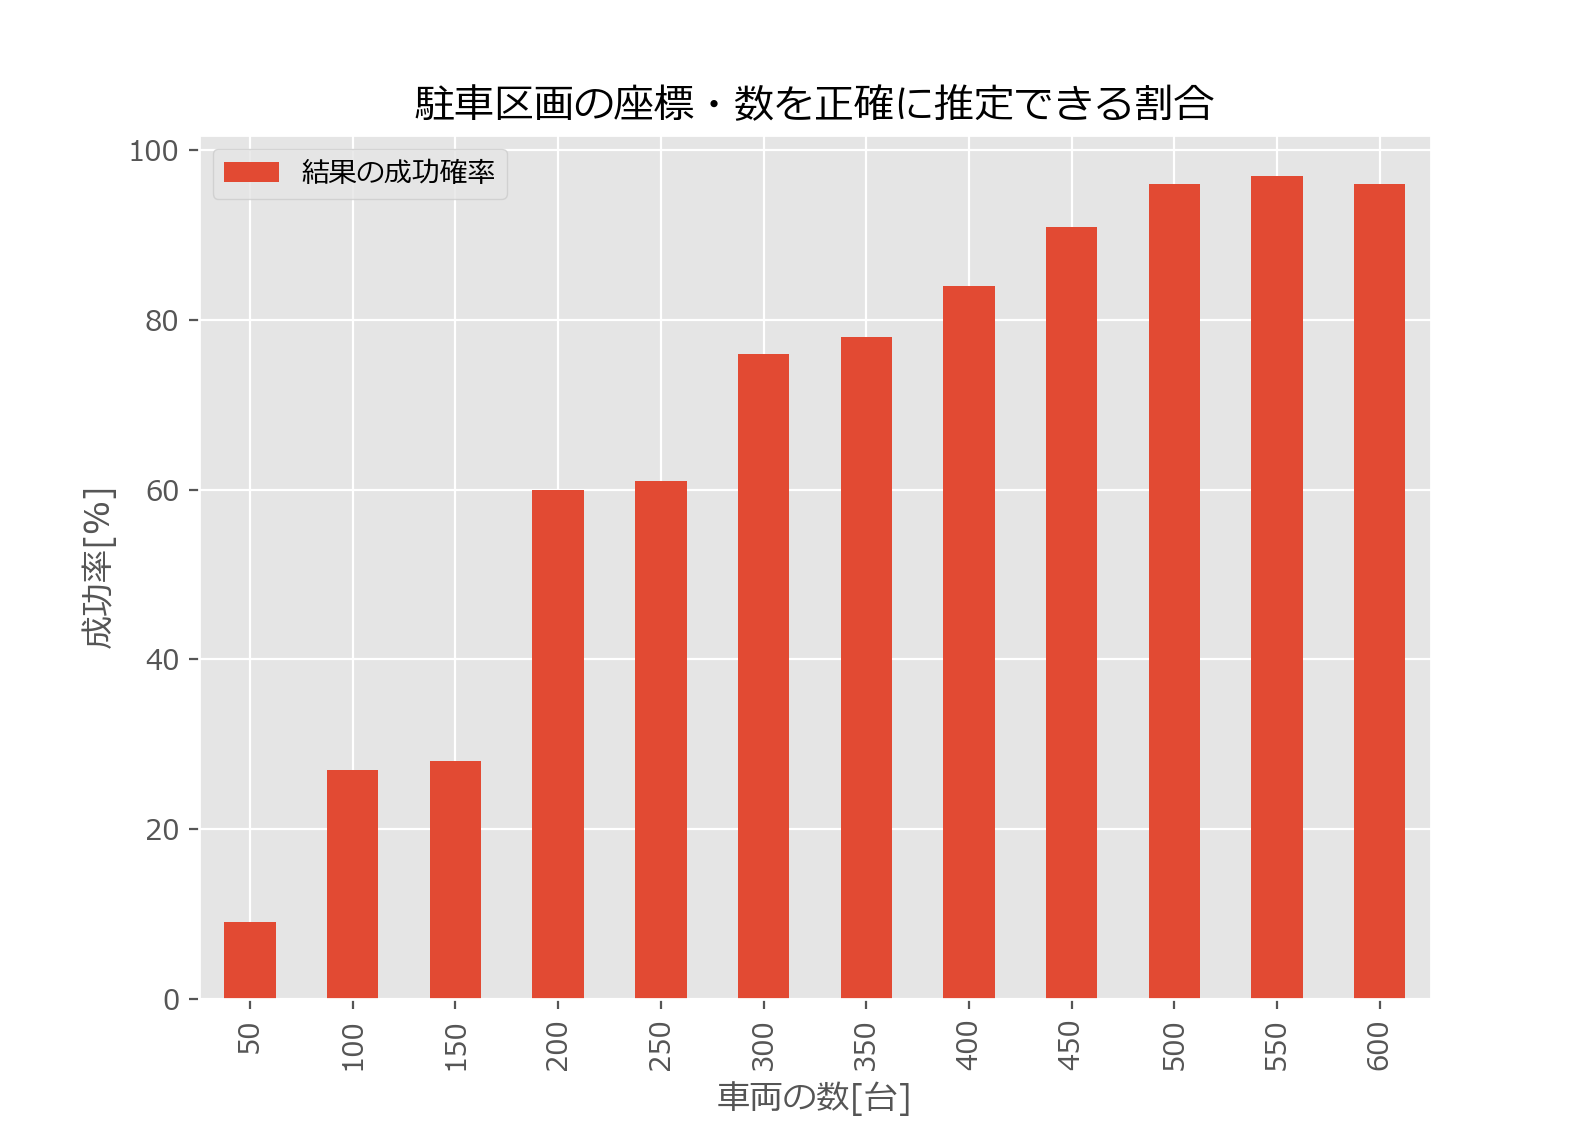
\includegraphics[width=14cm]{fig/evaluate-result.png}
	\caption{利用車両の台数と推定の成功率の関係性}
	\label{evaluation_test_result_figure}
\end{figure}


\subsubsection{考察}
第\ref{model-case}節より,本実験が対象としたSFCキャンパスの総駐車枠数は222[台]であるため,$90\%$以上の成功率を得るためには,総駐車枠の$200\%$以上の述べ車両台数が必要であることがわかった.1日のうちに駐車区画の多くが満車近くになるSFCの駐車場の場合,データ推定対象となる時間を2日以上に設定することで,十分に信頼できるネットワークモデル推定を行うことが出来ると言える.


\clearpage

\subsection{評価実験2:駐車区画が保有する駐車枠数の推定}
\label{evaluation-test-2}
本項では,第\ref{how-to-park-slot}節で述べた,駐車区画が保有する駐車枠数の推定手法を定量的に評価するための評価実験について記述する.

\subsubsection{条件と変数}
評価実験2では,第\ref{evaluation-test-conditions}節に挙げた条件の他に,以下のような条件を設定する.
\begin{itemize}
	\item 仮想車両のスタート方法\\
	      すべての車両を同時にスタート地点から進入させる.
	\item 最大シーケンス数(収集対象時間) \\
	      評価実験2では最大シーケンス数を設定しない.すべての車両が駐車を完了し,SFCから退出するまでの位置情報ログを本評価実験での推定に用いる.
	\item 車両台数 \\
	      \ref{evaluation-test-1-eval-elements}項で述べたように,評価実験1では,導入する車両台数に最大シーケンス数中の述べ車両台数という意味付けを行った.一方で,評価実験2では場内に存在する最大車両台数と換言する.
	\item 前提となる推定結果 \\
	      駐車枠数の推定を行うためには駐車区画の数$\cdot$座標の2項目が正しく推定されていることが必要である.よって,第\ref{evaluation-test-1-eval-elements}項で定めた基準を満たした場合の推定結果を前提条件とする.
\end{itemize}
\subsubsection{評価項目}
評価実験2では,以下の項目に関して推定結果を検証し,推定の妥当性を検証する.
\begin{enumerate}
	\item 充足率 \\
	      駐車区画$p$に関して,システムが推定した保有枠数$a_p$の真値$G_p$に対する割合を推定充足率$F_p = \frac{a_p}{G_p}$と定義する.$F_p = 1$の時,真値と同じ値を推定したと見なすことが出来る.なお,\ref{how-to-park-slot}項より,$a_p \leq G_p$であるため,$F_p \leq 1 $である.
\end{enumerate}


% 試行回数はn'にしたほうがいい気もする.前提条件があるので
\subsubsection{説明変数と目的変数}
評価実験2では,仮想地図内に進入する車両の台数を説明変数$x$とし,$n$回試行した際の,駐車区画$p$の推定充足率$F_{pn}$の中央値$\tilde{F_{pn}}$を目的変数$y_p$とする.なお,本実験において,$x = 50,100,150,200,250,300,350,400,450,500,550,600$,試行回数$n=100$とする.
\begin{align}
	y_p = \tilde{F}_{pn}                                   \\
	F_{pn} = n回試行した際の推定充足率群      \\
	F_p = \frac{a_p}{G_p}                                  \\
	f_{2}(x,p) = a_p \\
	f_{2}(x,p) = 本推定手法, x = 車両の台数,p = 駐車区画\\
	n = 総試行回数                                    
\end{align}
\subsubsection{結果}
本項では評価実験2の結果について述べる.推定された推定充足率の中央値$\tilde{F_{pn}}$と,車両数$x$との関係を図\ref{slot-result-all-mean-fig}に示す.図\ref{slot-result-boxplots}に各駐車枠ごとの結果を示す.


\begin{figure}[htbp]
	\centering
	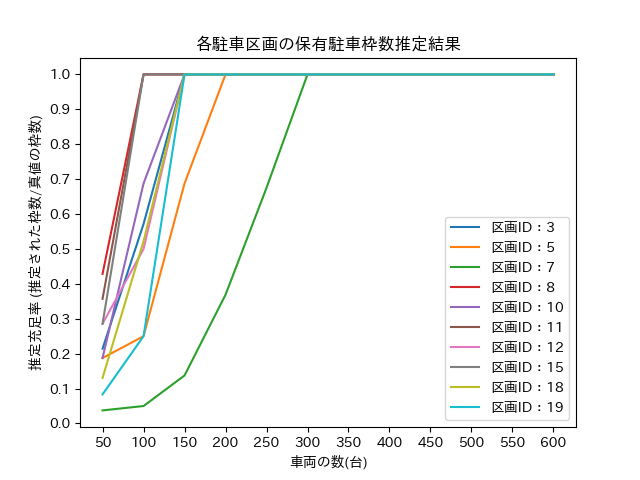
\includegraphics[width=14cm]{fig/slot-result-all-mean.png}
	\caption{仮想地図内の最大車両台数と各駐車区画の推定充足率}
	\label{slot-result-all-mean-fig}
\end{figure}

\begin{figure}
	\centering
	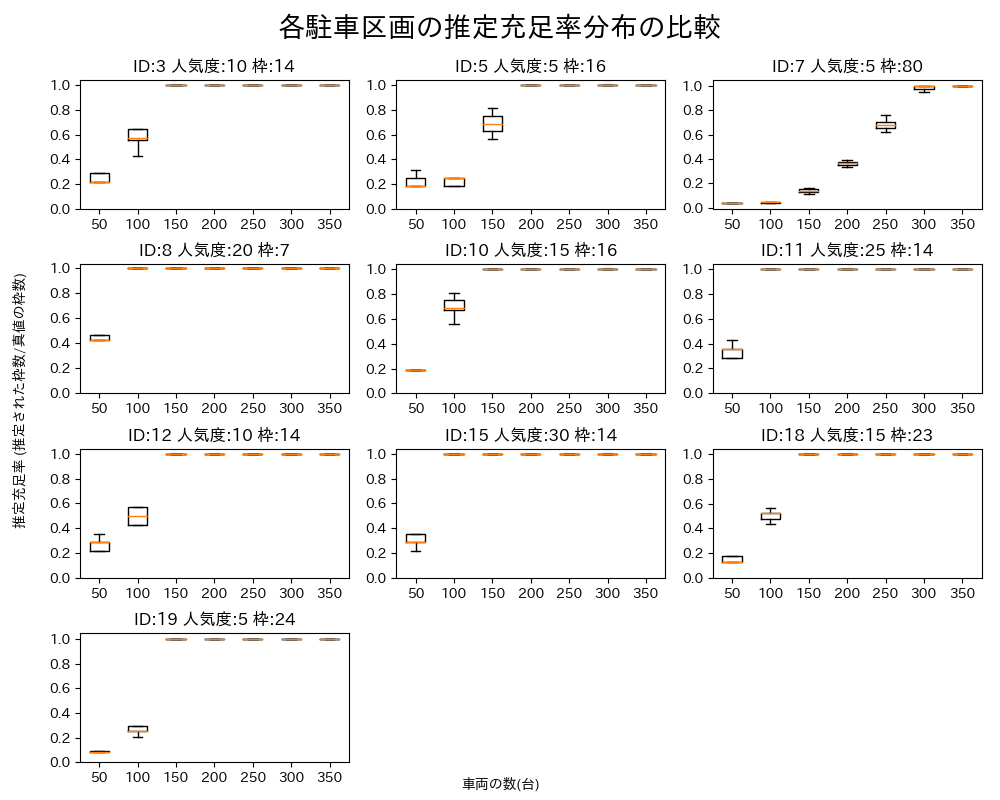
\includegraphics[width=16cm]{fig/slot-result-boxplots.png}
	\caption{仮想地図内の最大車両台数と各駐車区画の推定充足率}
	\label{slot-result-boxplots}
\end{figure}

\subsubsection{考察}
図\ref{slot-result-all-mean-fig}より,多くの駐車区画が$x>200$の時,駐車枠数の完全な推定に成功しているケースが多いことが読み取れる.また,人気度の低い2つの区画を除けば,$x>150$の時完全な推測に成功する可能性が高いことがわかる.第\ref{model-case}節より,本実験が対象としたSFCキャンパスの総駐車枠数は222[台]であるため,駐車場内の満車率が$70\%$程度になった場合に,主要な駐車区画の保有する枠数を推定できたと言える.


また,図\ref{slot-result-boxplots}より,区画ID:15やID:11のような特に人気が高い駐車区画に関しては,$x>100$の場合に推測に成功していると言える.人気度が特に高い駐車枠に限れば,満車率が$50\%$程度あれば枠数の把握が可能になることが導かれる.


しかしながら,区画ID:7では,駐車場の総枠数(222[台])以上に車両が場内に進入していても推定充足率が1に満たない.これは,空き枠のある駐車区画があるのにも関わらず,駐車場内を巡回している車両が多く発生していることを意味している.この現象は,各駐車区画の満空状況を各車両が走行中に把握することが出来ない(\ref{evaluation-test-conditions}節を参照)ことが原因であると考えられる.
本評価実験の結果より,人気度が低く枠数が多い駐車区画では,現実的な車両台数では推測できないことが明らかになった.